\documentclass[a4paper, fleqn]{article}

\usepackage{amsmath}
\usepackage{enumitem}
\usepackage{graphicx}

\begin{document}

\title{Homework III \\ Introduction to Physical Chemistry}
\author{Basil R. Yap 1001690}
\date{2018 February 08}
\maketitle

\section{Question 1}

\begin{enumerate}[label=(\alph{*})]
\item $\begin{aligned}E&=-(2.18\times10^{-18})\frac{Z^2}{n^2}\\&=-(2.18\times10^{-18})\frac{3^2}{1^2}\\&=-1.96\times10^{-17}J\end{aligned}$
\item \textbf{Figure 1}:\begin{figure}[h!]
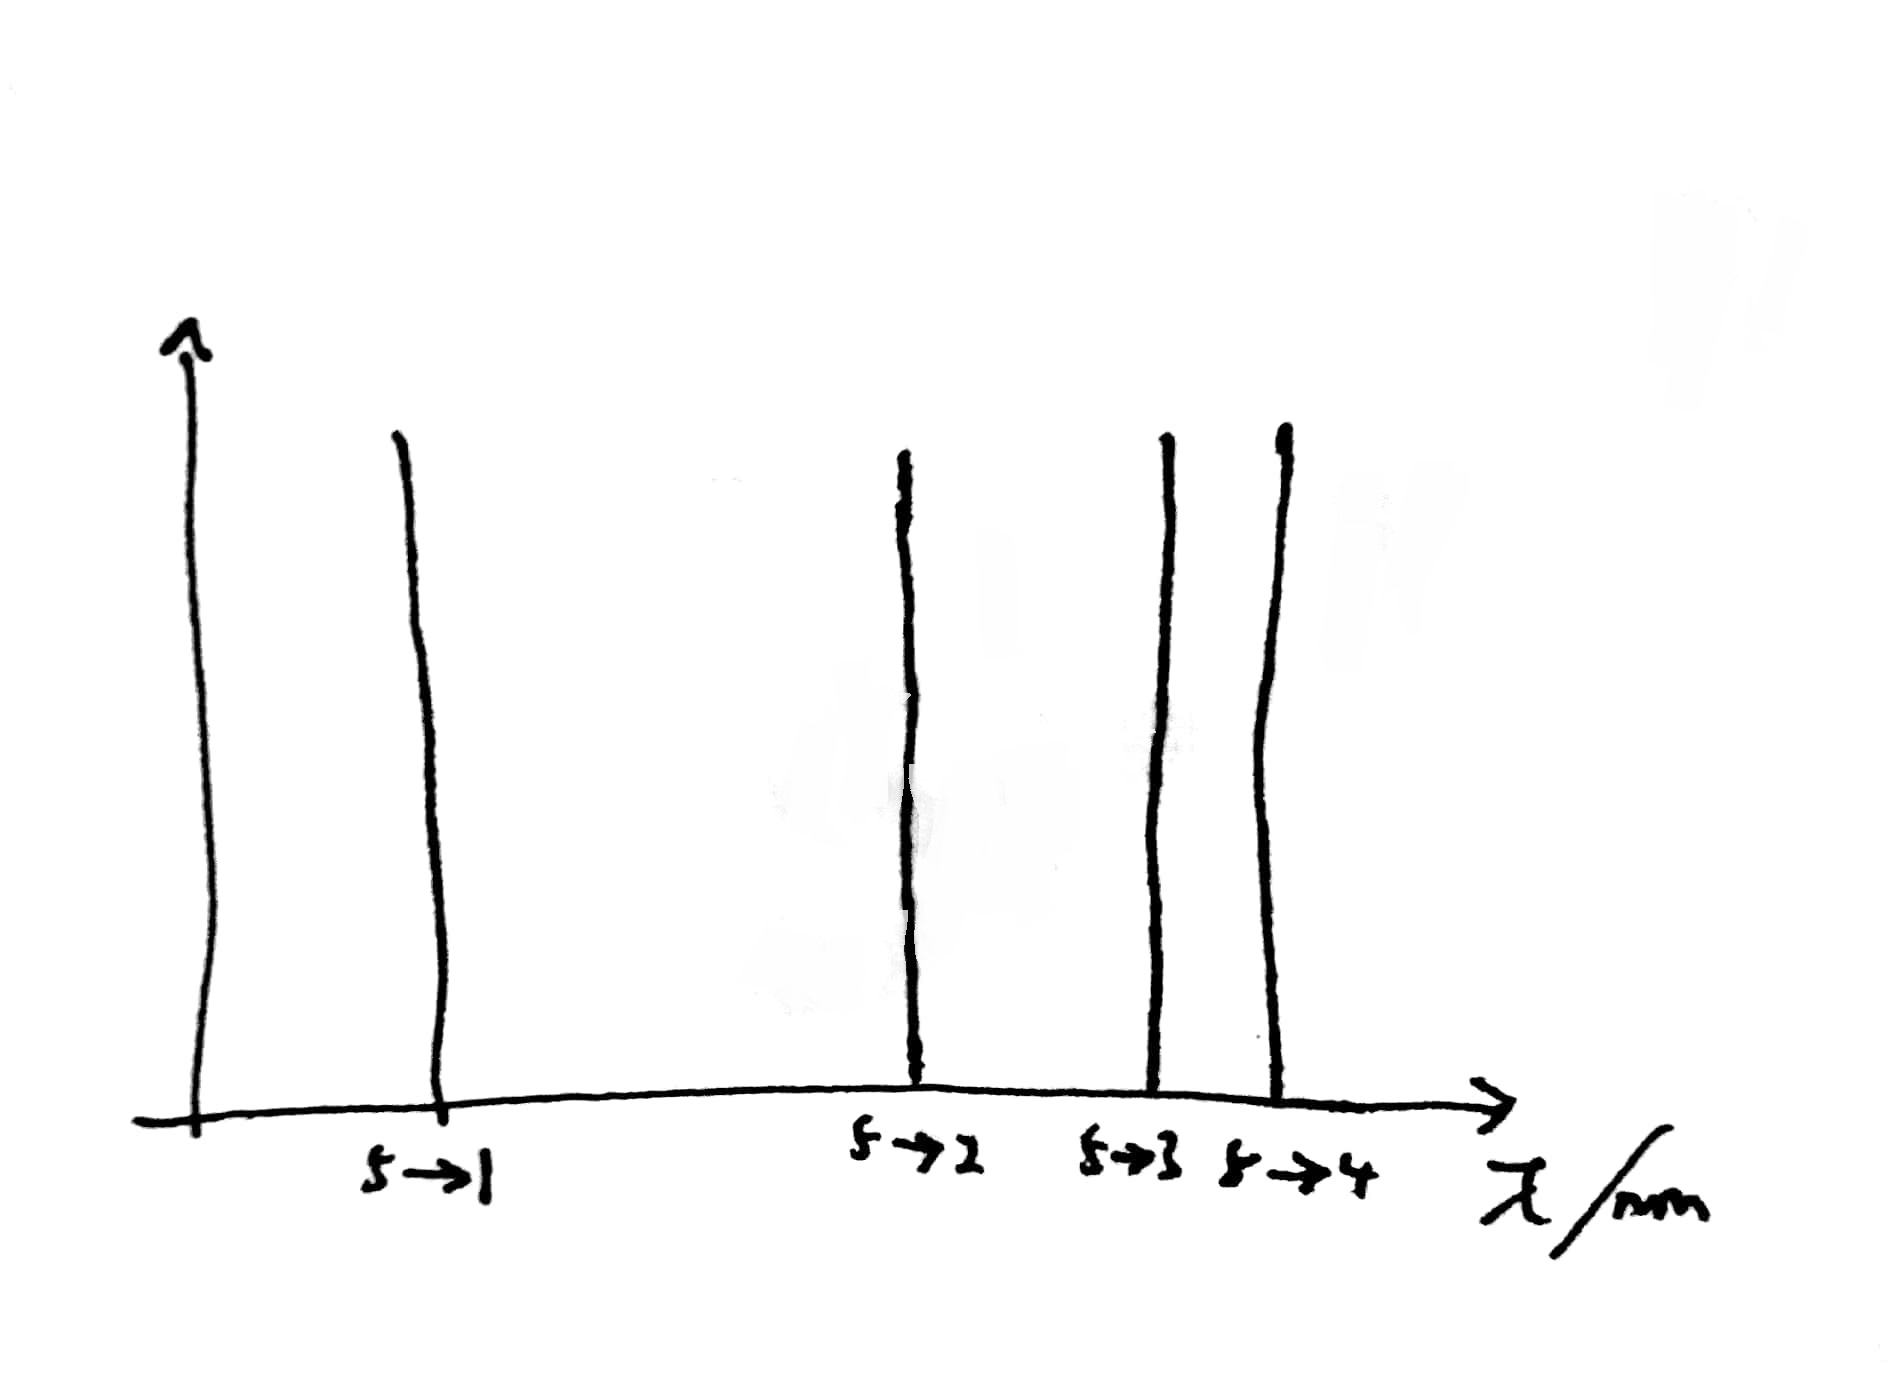
\includegraphics[width=\linewidth]{./assets/201802120749.jpg}
\caption{Line Spectrum}
\label{figure:graph1}
\end{figure}
\end{enumerate}
\pagebreak
\section{Question 2}
\begin{enumerate}[label=(\alph{*})]
\item $1s^1$
\item $\begin{aligned}E&=-(2.18\times10^{-18})\frac{Z^2}{n^2}\\&=-(2.18\times10^{-18})\frac{4^2}{3^2}\\&=-3.876\times10^{-18}J\end{aligned}$
\item $\begin{aligned}E&=hv\\v&=\frac{E}{h}\\&=\frac{3.876\times10^{-18}}{6.626\times10^{-34}}\\&=5.849\times10^{15}\text{Hz}\end{aligned}$
\item $\begin{aligned}E&=-(2.18\times10^{-18})\frac{Z^2}{n^2}\\&=-(2.18\times10^{-18})\frac{1^2}{3^2}\\&=-9.69\times10^{-19}J\end{aligned}$\\
The binding energy of a H electron is higher than that of a Be electron. This is because the nuclear charge of a beryllium ion is higher than the nuclear charge of a hydrogen ion, requiring more energy to remove an electron from the second excitation level.
\item This is an emission of a photon, as the electron goes from a lower potential energy level to a higher potential energy level.\\
$\begin{aligned}\Delta E&=-(2.18\times10^{-18})\left(\frac{Z^2}{n_1^2}-\frac{Z^2}{n_2^2}\right)\\&=-(2.18\times10^{-18})\left(\frac{4^2}{3^2}-\frac{4^2}{1^2}\right)\\&=3.1\times10^{-17}\\E&=\frac{hc}{\lambda}\\\lambda&=\frac{hc}{E}\\&=\frac{6.626\times10^{-34}\times2.99\times10^8}{3.1\times10^{-17}}\\&=6.39\times10^{-9}m\end{aligned}$
\end{enumerate}
\pagebreak
\section{Question 3}
\begin{enumerate}[label=(\alph{*})]
\item $\begin{aligned}KE&=\frac{hc}{\lambda}-\Phi\\&=\frac{6.626\times10^{-34}\times2.99\times10^8}{9.89\times10^{-10}}-\Phi\\&=2\times10^{-16}-\Phi\end{aligned}$
\begin{center}
\begin{tabular}{| c | c | c |}
\hline
Energy levels & $\Phi$ & KE\\
\hline
2s & 273 eV & $1.563\times10^{-16}$\\
2p & 205 eV & $1.672\times10^{-16}$\\
3s & 21 eV & $1.966\times10^{-16}$\\
3p & 10 eV & $1.984\times10^{-16}$\\
\hline
\end{tabular}
\end{center}
\begin{figure}[h!]
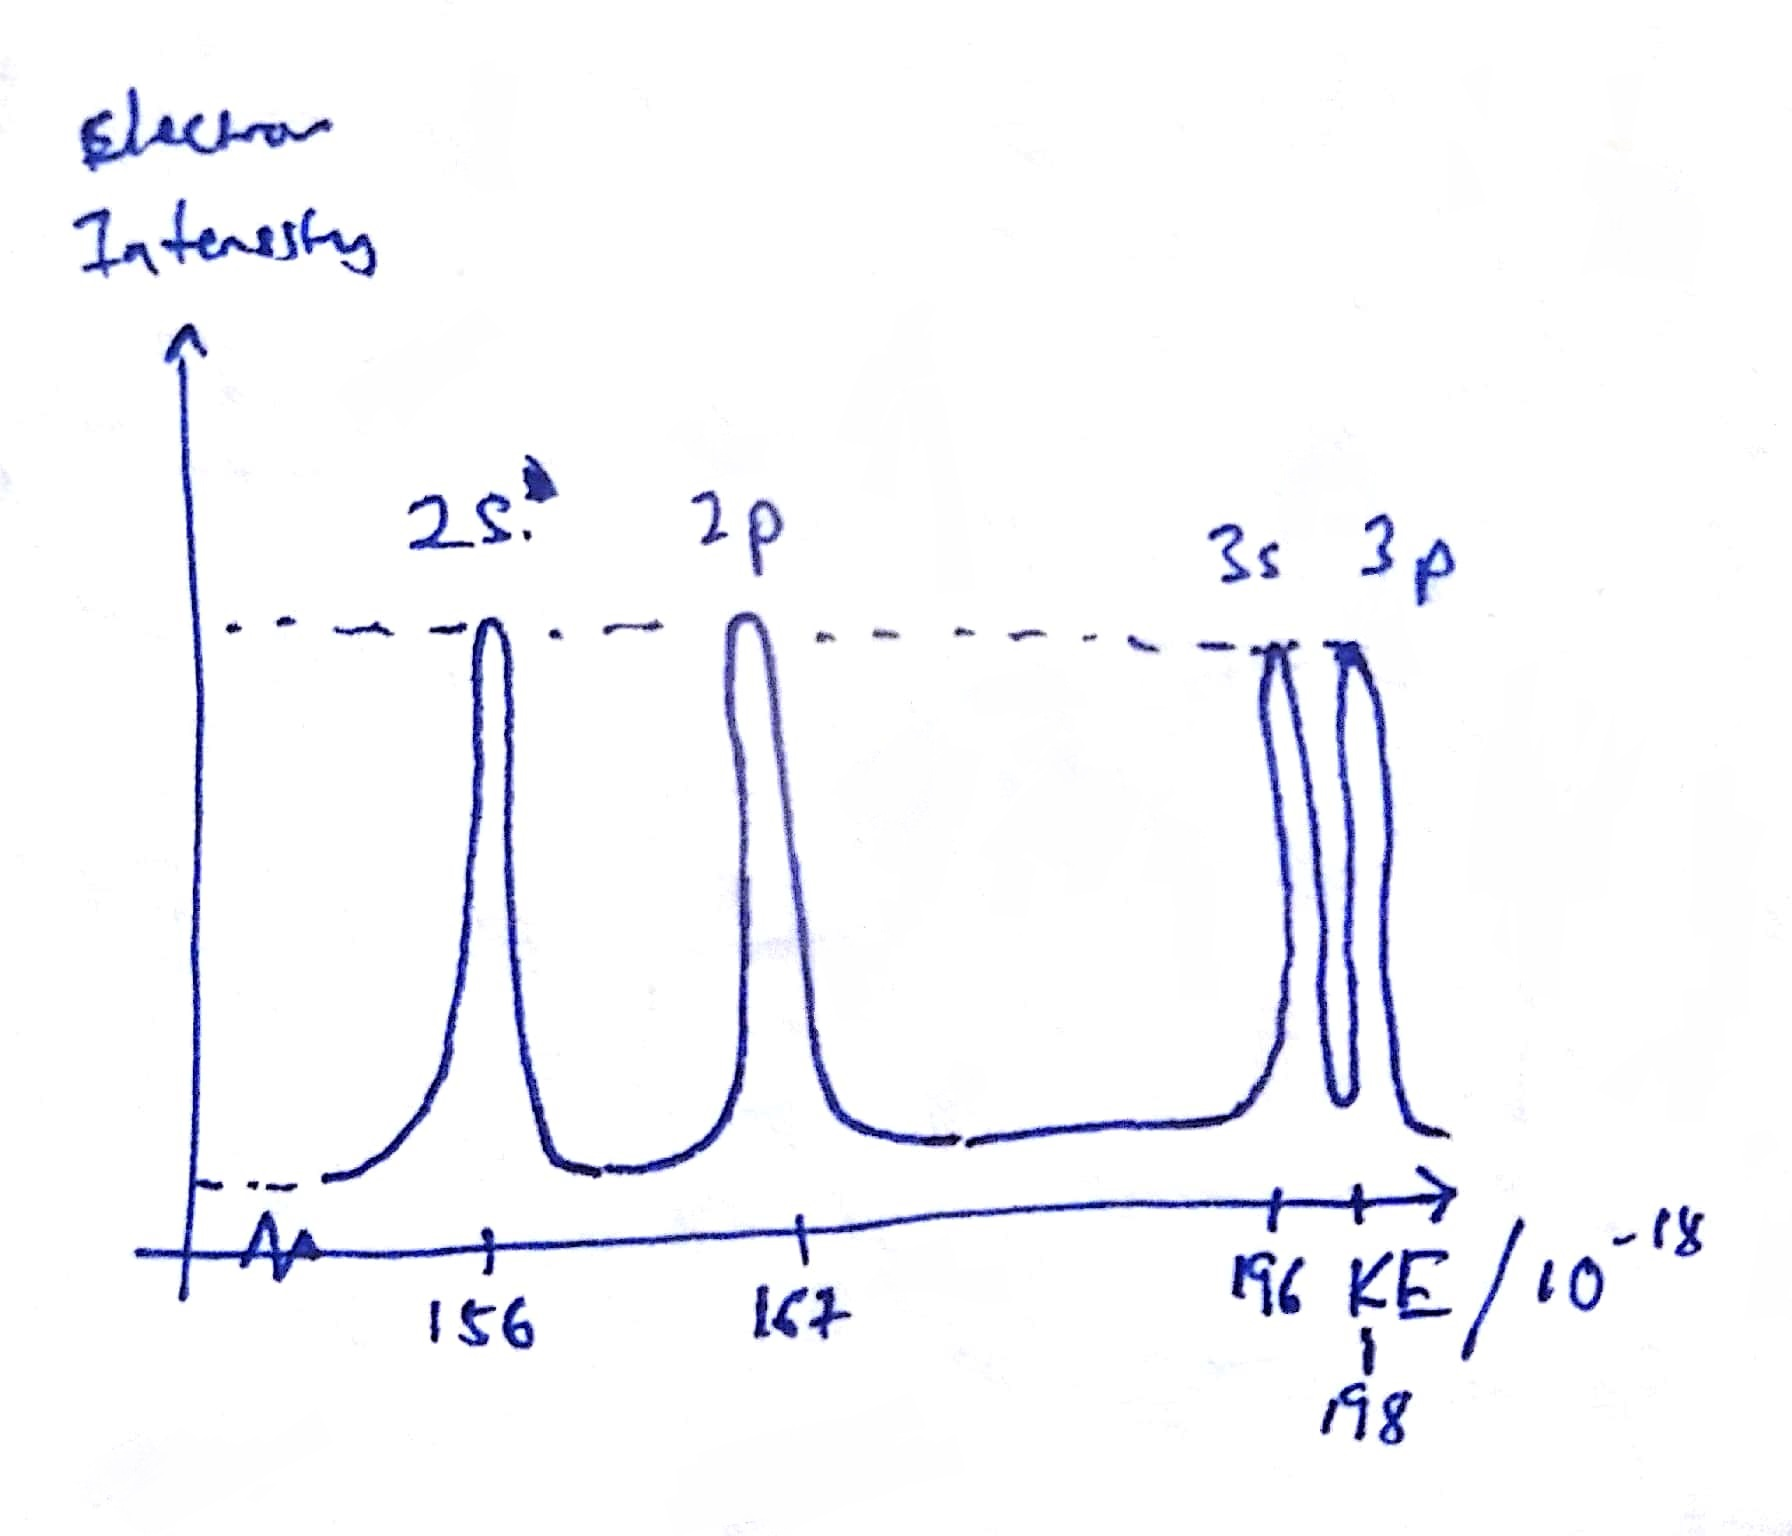
\includegraphics[width=\linewidth]{./assets/201802120534.jpg}
\caption{Stick Spectrum}
\label{figure:graph2}
\end{figure}
\item $\begin{aligned}Z_{eff}&=Z-S\\&= 17-10\\&=+7\end{aligned}$
\end{enumerate}
\pagebreak
\section{Question 4}
\begin{enumerate}[label=(\alph{*})]
\item \textbf{Figure 3}
\begin{figure}[h!]
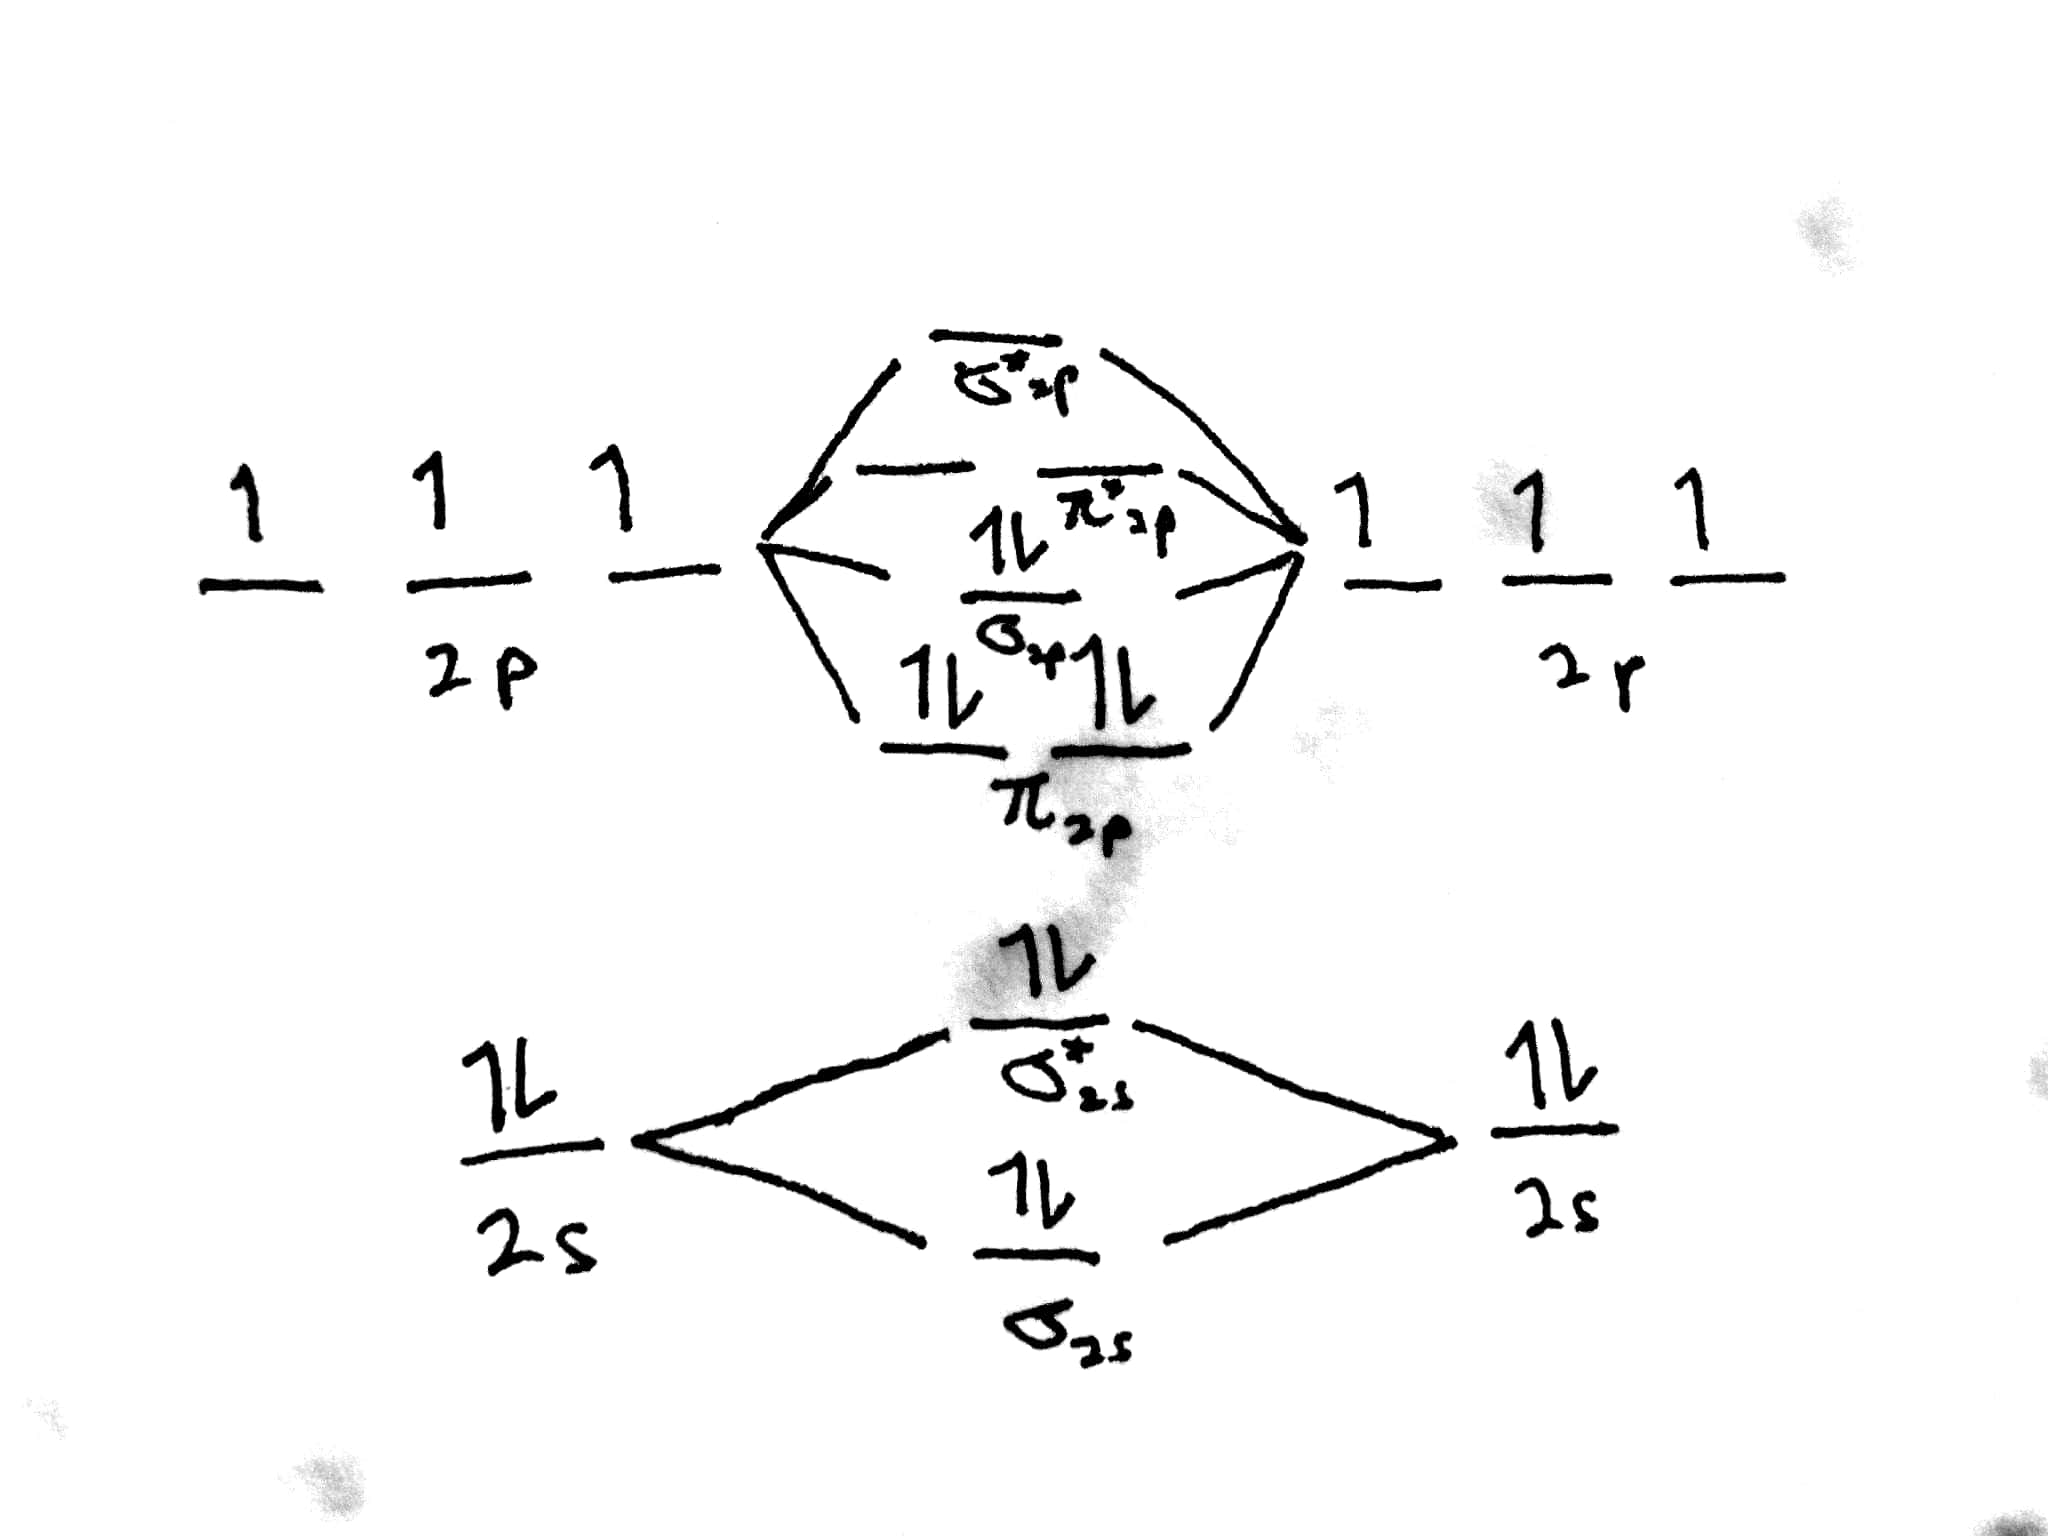
\includegraphics[width=\linewidth]{./assets/201802120600.jpg}
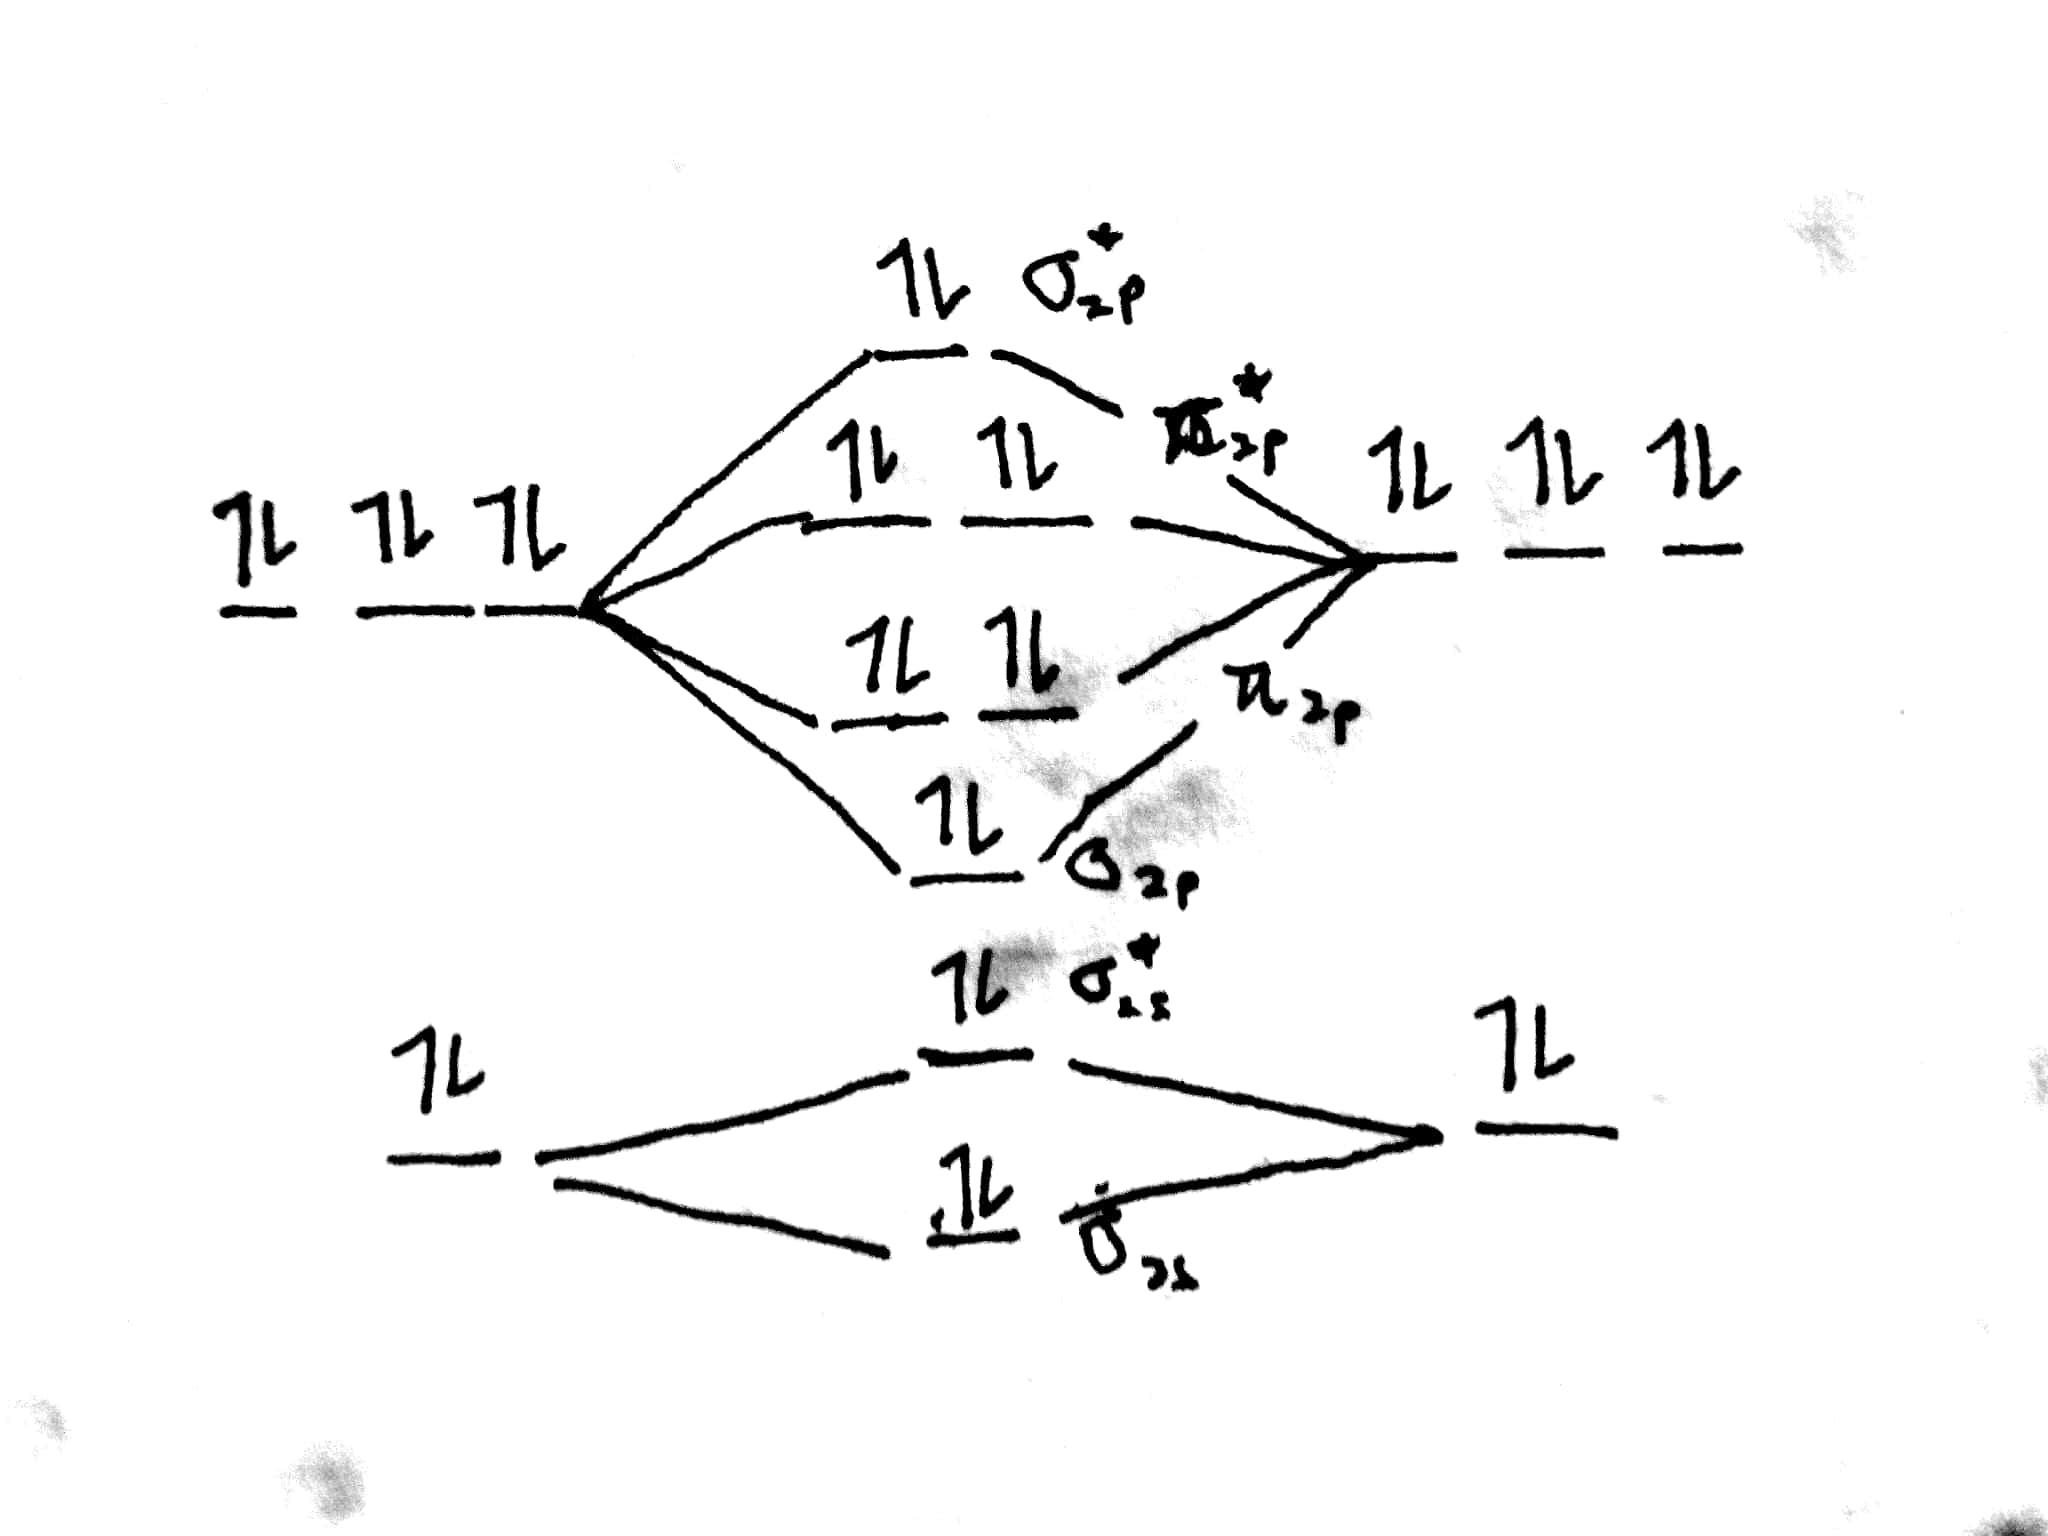
\includegraphics[width=\linewidth]{./assets/201802120606.jpg}
\caption{Molecular Orbital Diagram of N$_2$(above) \& Ne$_2$(below)}
\label{figure:graph3}
\end{figure}
\item \begin{itemize}
\item N$_2$: $(\sigma_{2s})^2(\sigma_{2s}^*)^2(\pi_{2px})^2(\pi_{2py})^2(\sigma_{2pz})^2$
\item Ne$_2$: $(\sigma_{2s})^2(\sigma_{2s}^*)^2(\sigma_{2pz})^2(\pi_{2px})^2(\pi_{2py})^2(\pi_{2px}^*)^2(\pi_{2py}^*)^2(\sigma_{2pz}^*)^2$
\end{itemize}
\item From the the MO Diagram, \begin{itemize}
\item N$_2$: 3
\item Ne$_2$: 0
\end{itemize}
N$_2$ is more stable than Ne$_2$ because it has a higher bond order. This is because both molecules have the same number of bonding orbitals but N$_2$ has fewer anti-bonding orbitals.
\item Yes, there is a difference between the positions of the $\sigma_{2p}$ and $\pi_{2p}$ orbitals of the two molecules. In N$_2$, the $\pi_{2p}$ orbital is at a lower energy level than $\sigma_{2p}$, and the opposite is true for Ne$_2$. This is due to a phenomena called s-p mixing, where molecules made of elements with lower nuclear charge have small differences in energy level between $\sigma_{2p}$ and $\pi_{2p}$. At higher nuclear charges, such as Ne, the difference becomes significant enough for the energy level of $\pi_{2p}$ to be higher than that of $\sigma_{2p}$
\end{enumerate}

\section{Question 5}
\begin{enumerate}[label=(\alph{*})]
\item \begin{itemize}
\item A: B
\item Bond order = 1.5
\end{itemize}
\item \begin{itemize}
\item D: Be
\item Bond order = 0
\end{itemize}
\item \begin{itemize}
\item E: F
\item Bond order = 2
\end{itemize} 
\end{enumerate}
\pagebreak
\section{Question 6}
\begin{enumerate}[label=(\alph{*})]
\item \textbf{Figure 4}:\begin{figure}[h!]
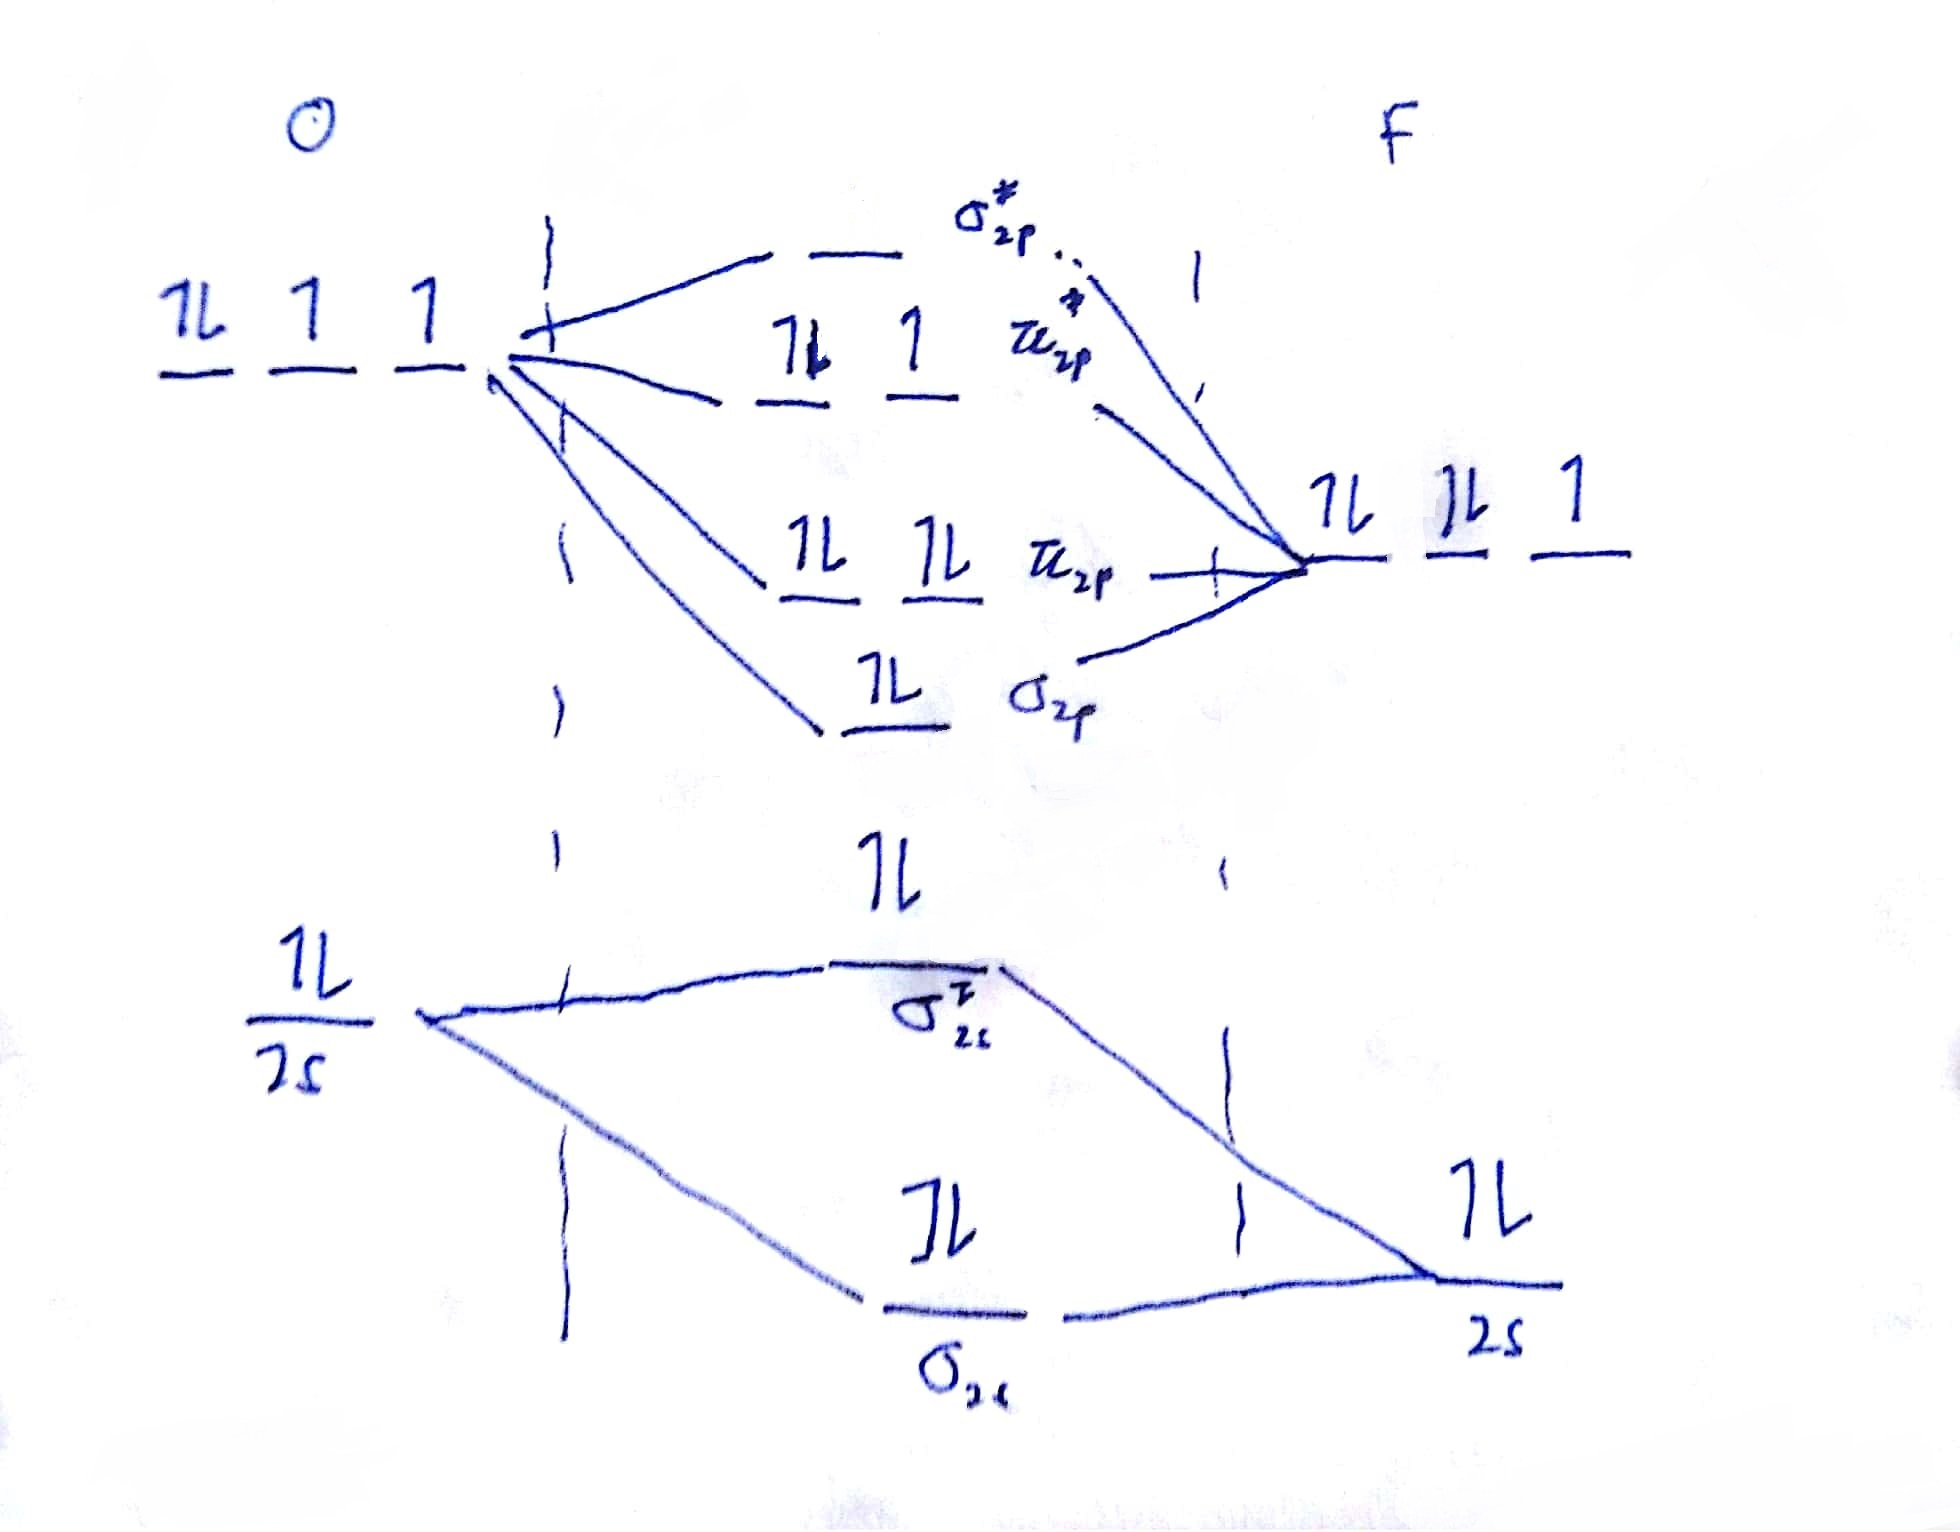
\includegraphics[width=\linewidth]{./assets/201802120711.jpg}
\caption{MO Diagram of FO}
\label{figure:graph4}
\end{figure}
\item The MO bond order of OF = 1.5
\item The MO bond order of OF$^+$ = 2\\
The bond shortens because the electron in the $\pi_{2px}^*$ orbital is removed, reducing the number of electrons populating the anti-bonding orbitals by one, thereby increasing the bond order and decreasing the bond length.
\item \begin{itemize}
\item HOMO: $\pi_{2px}^*$
\item LUMO: $\sigma_{2pz}^*$
\end{itemize}
\item Paramagnetic
\end{enumerate}

\end{document}